The CMP model treats the heart as homogeneous on large scales with a constant fibre orientation, and assumes that the heart is shaped like a cylindrical shell. This means it cannot reproduce phenomena that are dependent on large-scale heterogeneity or specific anatomical features, which severely limits its clinical applications. Our novel generalisation of the CMP model to include both large-scale heterogeneity and anatomical features is therefore an important extension to the model.

% This particular 

\section{Sheep Heart Data}

We were provided with a sheep atrium fibre map by \etalcite{zhao}{Zhao}
in the form of a discrete 3-dimensional vector field. At each point in this vector field, there is a direction vector that represents the prevailing muscle fibre direction in a $50~\mathrm{\mu m} \times 50~\mathrm{\mu m} \times 50~\mathrm{\mu m}$ cube (or `voxel') centred on that point. If the direction vector for a particular voxel is the zero vector, there is no atrial muscle in that voxel. The magnitude of the direction vector has no biological relevance (unless it is zero), so we normalised the non-zero direction vectors before proceeding.


\section{Model Preparation}

To convert the sheep heart fibre map to a usable format, we applied fibre tracking algorithms to reconstruct the muscle fibres of the heart, giving a network embedded in 3D space.
Generating the network is a multi-step, computationally intensive process. The final procedure is outlined in the following subsections, and the choices made are justified at the end of this section. A small section of one such network is shown in Fig.~\ref{fig:sample}, for illustrative purposes.

It should be noted that the network we produced was not the same as the original sheep heart; the fibre map does not contain sufficient information to do this~\cite{jiang2006dtistudio}. However, our network reproduces the anisotropy of the network and includes key anatomical features like the pulmonary veins.

\begin{figure} \begin{mdframed}
    \centering
    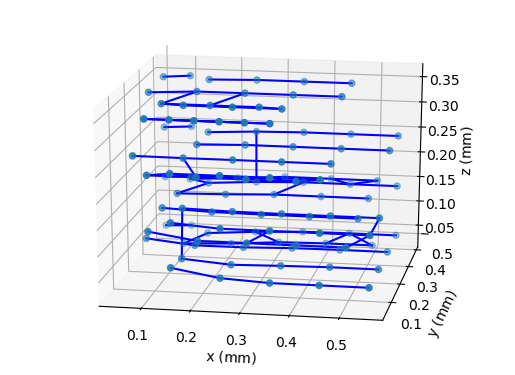
\includegraphics[width=0.7\textwidth]{sample}
    \caption{A small section of a finished network. Each point is a site that obeys the rules of the CMP model, and each line between sites represents a connection. In this example the fibres mostly lie along the x-axis.}
    \label{fig:sample}
\end{mdframed} \end{figure}

\subsection{Coarse Graining}

In order to make the network generation computationally feasible, the vector field was first coarse-grained. For a coarse graining factor of $g$, this meant taking the sum of all vectors in each separate $g \times g \times g$ cube in the original vector field, then normalising the new vector to have unit length. This reduced each linear dimension by a factor of $g$ and the total volume by $g^3$. We took $g = 6$ in order to attain the computational speed necessary for good statistics, whilst retaining as much anatomical detail as possible.

When we change the model dimensions in this way, we are decreasing the length scale of the model by a factor of $g$. However, the real time required for a signal to cross the atrium must remain the same, so we have to decrease the time scale of the model by a factor of $g$ (thus reducing the refractory period and pacemaker period). This means that the conduction velocity is unchanged by coarse graining.

\subsection{Fibre Tracking}

We have chosen to adapt the Fibre Assignment by Continuous Tracking (henceforth called `FACT') algorithm, which was developed for reproducing networks of the brain from MRI data and is well-established in the field of neuroscience~\cite{fact, bello2008motor}. The algorithm produces a fibre given a vector field, and works as follows~\cite{fact}:
\begin{enumerate}
    \item Pick a point to be a `seed point'. We used the centre of each non-empty voxel.
    \item Find the direction of the vector field in the voxel containing that seed point, and then follow this vector field until reaching the boundary of this voxel with another voxel. Store the coordinates of this intersection.
    \item Find the direction vector in this other voxel and then follow that until reaching a boundary with another voxel. Store the coordinates of this intersection. Keep repeating this process until one of the following termination conditions is met:
    \begin{enumerate}
        \item An empty voxel is reached (i.e. a voxel where the direction vector is zero).
        \item The fibre encounters a sharp turn, i.e. a turn where the angle between previous direction of the fibre and the new direction of the fibre is greater than $\sim 40 \degree$.
        \item The fibre reaches a certain length. We chose a length of $8~\mathrm{mm}$, as this is approximately the length of fibres in the human heart~\cite{schwinger1994failing}. Obviously there will be differences between a sheep heart and a human heart but it is likely that these lengths are similar enough for our purposes to provide an approximate estimate.
    \end{enumerate}
\end{enumerate}
For each seed point, we first followed the vector field forwards, then we followed it backwards. Our maximum-length termination condition was applied to both halves of the fibre separately, so the maximum length of a fibre in our model was actually $2 \times 8~\mathrm{mm}$. This is still acceptable because $8~\mathrm{mm}$ was only an approximate estimate. This gave us a list of points that defined a fibre. A simplified 2D version of this process is detailed in Fig.~\ref{fig:fact}.

We repeated the above process for every single non-empty voxel, giving a huge number of fibres. However, this resulted in two problems:
\begin{itemize}
    \item The fibres had unevenly spaced points because the fibre was defined by the list of intersections with voxel boundaries (see Fig. \ref{fig:fact}). The rules of the CMP model dictate that a signal can cross one connection between sites in one timestep. This meant that the conduction velocity was slower when points were close together and faster when they were far apart. We needed fibres to conduct at a uniform speed along their entire length.
    \item For each non-empty voxel in the vector field, we had a fibre. This led to a density of fibres that is both non-uniform and far higher than what is seen in the real heart.
\end{itemize}

\begin{figure} \begin{mdframed}
    \centering
    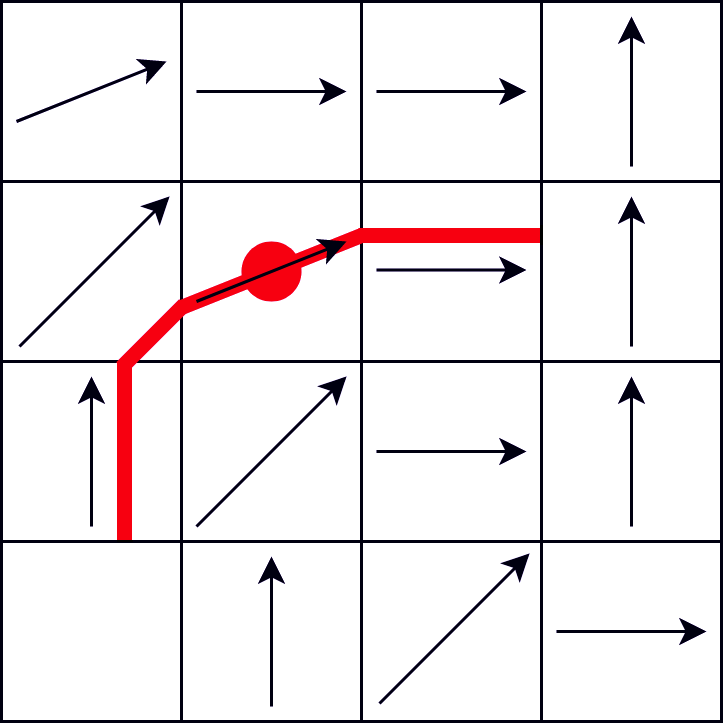
\includegraphics[width=0.7\textwidth]{fact}
    \caption{Behaviour of FACT algorithm in 2D. The black arrows indicate the vector field (i.e. the prevailing directions of the fibres). The large red dot is the starting position of the fibre tracing. From there, the vector field is traced both forwards and backwards. The tracing follows the field in a straight line until it reaches a boundary, and then it follows the new direction until it reaches the next boundary, and so on. We store all the intersections of the fibres with the voxel boundaries, and these define a fibre.
    The fibre is terminated when it reaches an empty square (lower left) or a sharp turn (upper right).}
    \label{fig:fact}
\end{mdframed} \end{figure}

\subsection{Interpolation}

To solve the problem of uneven conduction velocity, we interpolated along the fibres and placed points at equal distances along the fibre. To do this, we used the following algorithm:
\begin{enumerate}
    \item Let the position of the $i$th point along the fibre (counting from $i=0$ at one end of the fibre) be the vector $\mathbf{F_i}$.
    \item Calculate the cumulative distance along the fibre at each point. Let the $i$th cumulative distance be $C_i$. We define $C_0 = 0$, so for example $C_1 = \left| \mathbf{F_1} - \mathbf{F_0} \right|$ and $C_2 = C_1 + \left| \mathbf{F_2} - \mathbf{F_1} \right|$.
    \item To place a point a distance $x$ along the fibre, find the largest $C_i$ that is less than $x$, and note its index $i$. This was done using a binary search as the list of cumulative lengths is sorted by definition. This reduces the search time for a fibre with $N$ points from $\sim N$ (for a naive linear search) to $\sim \log(N)$; a significant improvement, especially for large fibres.
    \item Compute the vector: \begin{equation}
        \mathbf{F_i} + \frac{\mathbf{F_{i + 1}} - \mathbf{F_i}}{ \left| \mathbf{F_{i + 1}} - \mathbf{F_i} \right|} (x - C_i).
    \end{equation}
    This is the position of the point a distance $x$ along the fibre.
\end{enumerate}
For every fibre, we calculated a set of interpolated points with separation of 1 unit, corresponding to a real physical length of $g \times 50~\mathrm{\mu m}$. This ensured that points along the fibre were regularly spaced, thus solving the issue of irregular conduction velocity along fibres.

\subsection{Fibre Density Regulation}

To solve the problem of the fibre density being too high, we adapted the Spherical-deconvolution Informed Filtering of Tractograms (henceforth SIFT) algorithm, also well-established within the field of neuroscience~\cite{sift, stampfli2019subtle}. Since we don't have the information about how the actual fibre density varies throughout the heart, we have assumed that the density is uniform.

Our adapted SIFT algorithm involves minimising a cost function $c$:
\begin{equation}
    c = \frac{1}{L} \sum_{\mathrm{voxels}} (l_v - \Bar{l}),
\end{equation}
where $L$ is the total length of all fibres, $l_v$ is the total fibre length in a specific voxel $v$, and $\Bar{l}$ is the target length per voxel. 

To minimise this function, we calculated the change to the cost function $\Delta c$ if each fibre were deleted. Then, we picked the fibre that has the highest $\Delta c / l_f$, where $l_f$ is the total length of the fibre. Long fibres go through many voxels and therefore will reduce the cost function more than short fibres; considering $\Delta c / l_f$ rather than $\Delta c$ ensured that the algorithm was not biased towards removing long fibres~\cite{sift}. This process was repeated, removing fibres until the cost function reached a target value. Once this was done, we had a set of fibres with roughly uniform density.

\subsection{Transverse Connectivity}

Finally, we can add `transverse' connections between nodes in adjacent fibres. To do this, we define a connection probability function. This is a sigmoid function, which can be thought of as a smoothed-out step function:
\begin{equation}
    p_\text{conn}(r) = \frac{1}{e^{b(r - \mu)} + 1},
    \label{eq:pconn}
\end{equation}
where $r$ is the distance between nodes, $b$ is the steepness of the transition region, and $\mu$ is a characteristic distance that controls where the centre of the step is. We chose $b = 7$ as it caused $p_\text{conn}$ to drop off quickly enough with $r$ that it rarely connected non-adjacent fibres.
This functional form is acceptable as it is $1$ for small $r$ but rapidly drops to $0$ once $r > \mu$.
A plot of $p_\text{conn}(r)$ is shown in Fig.~\ref{fig:pconn}.

\begin{figure}[h] \begin{mdframed}
    \centering
    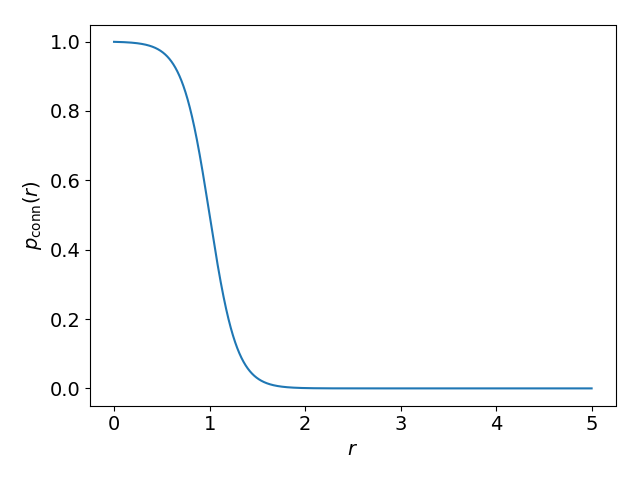
\includegraphics[width=0.7\textwidth]{pconn}
    \caption{The connection probability function for $\mu=1$, plotted as a function of distance between nodes $r$. The function rapidly declines after reaching $r > \mu$. Units are defined such that the voxel side length is unity.}
    \label{fig:pconn}
\end{mdframed} \end{figure}

Calculating $p_\text{conn}$ for every pair of points would cause the time for completion (assuming $N$ nodes in the model) to scale with $N^2$, which is unacceptably slow for large $N$. To improve this, we stored a list of the nodes in each voxel. Then, when adding connections between nodes, we could consider the set of nodes in only nearby voxels without having to compute $r$ for every pair of nodes. This brings the time required to be approximately linear in $N$.

$\mu$ is analogous to the parameter $\nu$ in the original CMP model; by varying it, the connectivity between fibres changes. This means decreasing $\mu$ is also analogous to increasing fibrosis. The presence of this parameter makes it possible to reproduce the results of the original CMP model using our generalised model.

Note that by repeating this process of adding transverse connections but changing the initial state of the pseudorandom number generator, different networks could be generated for a single $\mu$ value. This enabled collection of better statistics.

\subsection{Justification}

\subsubsection*{Oblique Conduction Velocity}

We have made the deliberate choice to avoid aligning our nodes to a Cartesian grid.
This approach has benefits over a naive 3D generalisation of the CMP model in which nodes are aligned to a cubic lattice, because it allows for uniform conduction velocity along the fibres, regardless of the fibre direction. Figure~\ref{fig:staircase} illustrates how the naive approach leads to the problem of different conduction velocities in the oblique and cardinal directions. 

% Our approach also allows faithful reconstruction of the anisotropy of the sheep atrium, which can be only loosely approximated by the naive approach. This is because on a grid there are only a few possible directions that connect adjacent nodes.

\begin{figure}[H] \begin{mdframed}
    \centering
    \begin{subfigure}[b]{0.46\textwidth}
        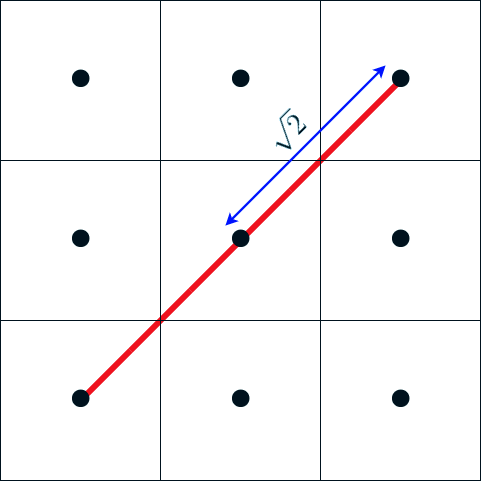
\includegraphics[width=\textwidth]{staircase_oblique}
        \caption{$45\degree$ connections allowed}
    \end{subfigure}
    ~
    \begin{subfigure}[b]{0.46\textwidth}
        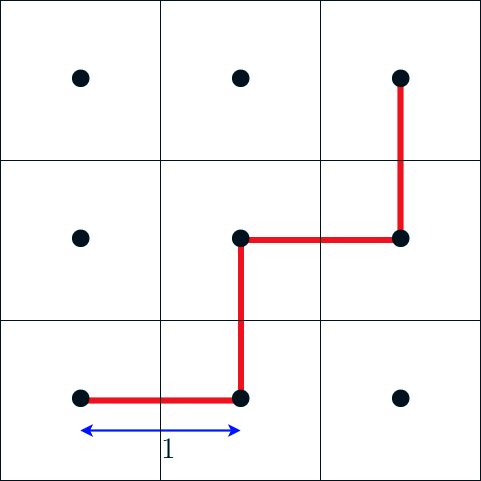
\includegraphics[width=\textwidth]{staircase_cardinal}
        \caption{$45\degree$ connections forbidden}
    \end{subfigure}
    \caption{The rules of the CMP model dictate that a signal crosses a connection (red) between two cells (black dots) in one timestep. In the cardinal directions we will therefore see a conduction velocity of one grid unit per timestep. However, in oblique directions the conduction velocity varies, which presents a problem: rotating the coordinate system would change the dynamics. This problem is illustrated under two possible rulesets for adding connections: in (a) $45\degree$ connections are allowed, and the conduction velocity in the oblique $45\degree$ direction is $\sqrt{2}$ grid units per timestep. In (b) we forbid oblique connections and the conduction velocity in the oblique direction is $\sqrt{2} / 2$ grid units per timestep. Neither of these are the same as the conduction velocity in the cardinal directions.}
    \label{fig:staircase}
\end{mdframed} \end{figure}

\subsubsection*{Why FACT and SIFT?}

This process was not the only one we tried; many weeks were required to settle on this process. The first process we tried was as follows:
\begin{enumerate}
    \item Pick an empty voxel (i.e. a voxel through which there are no fibres) and use as a seed point for FACT; fibres terminate if they enter a non-empty voxel, as well as if any of the previous termination conditions are met.
    \item Repeat for every empty voxel.
\end{enumerate}
However, this gave rise to unacceptable density variations depending on the orientation of the vector field, for reasons explained by Fig.~\ref{fig:firstattempt}. Variations in density will cause there to be more transverse connections in one place than another, which affects re-entry circuit formation and biases re-entry circuits to certain locations. Efforts to adapt $p_\text{conn}$ to correct for this bias were unsuccessful, so this approach had to be abandoned.

\begin{figure}[h] \begin{mdframed}
    \centering
    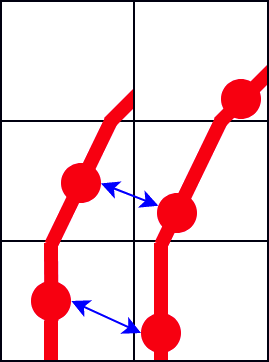
\includegraphics{firstattempt}
    \caption{An example of how our first attempt at producing a set of fibres from the atrial map can go wrong. Notice how the upper blue arrow (representing a potential transverse connection) is much shorter than the lower one. This happened because of a change in fibre direction, which is clearly unreasonable; the heart should not become more muscular in areas where the fibres are not aligned with the axes. Note that the left fibre has been terminated because it entered the same voxel as the right fibre.}
    \label{fig:firstattempt}
\end{mdframed} \end{figure}

We would expect the number of connections a node has to be approximately equal regardless of the direction of the fibre it lies upon. Figure~\ref{fig:angulardep} shows how the number of connections varies as a function of the angle between the fibre direction and the x-y plane, for both the FACT/SIFT approach, and this simpler approach.

\begin{figure}[h] \begin{mdframed}
    \centering
    \begin{subfigure}[b]{0.8\textwidth}
        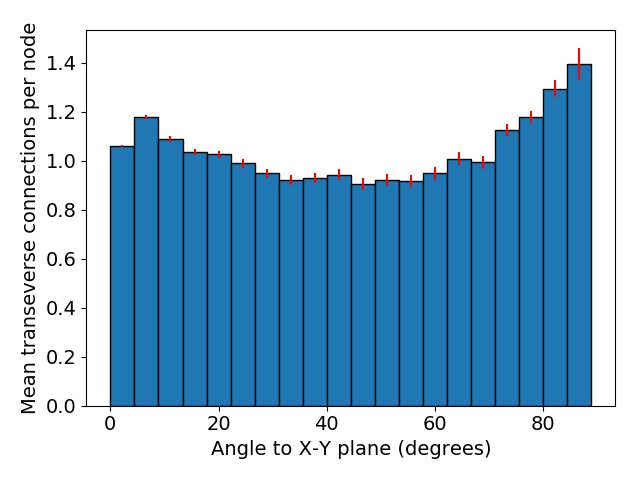
\includegraphics[width=\textwidth]{angular_connectivity_original}
        \caption{Our first attempt}
    \end{subfigure}
    
    \begin{subfigure}[b]{0.8\textwidth}
        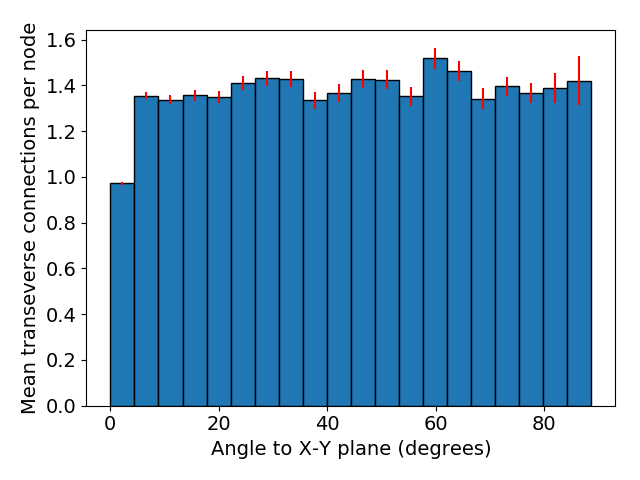
\includegraphics[width=\textwidth]{angular_connectivity_factsift}
        \caption{FACT/SIFT procedure}
    \end{subfigure}
    \caption{The connectivity of nodes as a function of fibre orientation. It can be seen that the FACT/SIFT approach gives a much more uniform connectivity (and therefore fibre density). The first attempt clearly shows that at oblique angles, the connectivity becomes lower, implying that the fibre density is also lower. The error bars (red) are the standard error of the mean. The drop for an angle of zero appears to be an artefact of the fibre map, as it appears under all our fibre tracking approaches.}
    \label{fig:angulardep}
\end{mdframed} \end{figure}

The main drawback to the FACT/SIFT approach is that the SIFT algorithm is extremely computationally intensive. Each time a fibre is removed, the quantity $\Delta c$ must be recalculated for every fibre, which scales with the number of fibres multiplied by the length of each fibre. However, SIFT is still faster than competing algorithms and avoids many of the same biases~\cite{sift}.

\clearpage
\section{Cell Behaviour}

The behaviour of individual cells is identical to the behaviour in the CMP model (summarised in Fig.~\ref{fig:cmpalgo}); we designated the same fraction (5\%) of cells defective, and they failed at the same rate (5\%). However, the pacemaker cells are now a small cluster in the right atrium, in the position of the sinoatrial node in the real heart. We designate any cells within a radius of 5 (corresponding to a distance of $5g \times 50~\mathrm{\mu m}$) of this point as pacemakers.
% TODO fill out the region

Note that in this generalised model, re-entry circuits form around anatomical obstacles in the same way as in the CMP model (previously explained in Fig.~\ref{fig:cmpreentry}). However, they can be significantly longer and more complicated. An example re-entry circuit from this generalised model is shown in Fig.~\ref{fig:newreentry}.

\begin{figure}[H] \begin{mdframed}
    \centering
    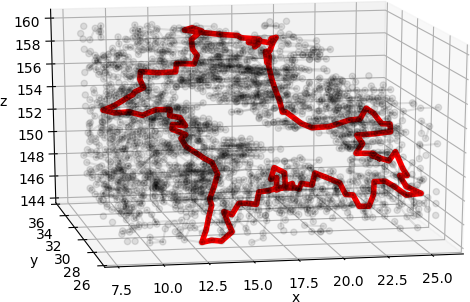
\includegraphics[width=1.0\textwidth]{circuit_example}
    \caption{An example of a re-entry circuit from the sheep atrium model, highlighted in red. The circuit has formed around a large empty region, which constitutes an anatomical obstacle. Note that this shows only a small subsection of the network. Axis units are in voxel coordinates.}
    \label{fig:newreentry}
\end{mdframed} \end{figure}

\clearpage 
\section{Results and Discussion}

This section presents the results of the generalised model. All results shown in this section are based on 1,000 different networks for each value of $\mu$, unless otherwise stated. Coarse graining of $g=6$ is used throughout.

\subsection{Risk Curve}

A necessary verification of this model is to produce a risk curve (first shown for the 2D CMP model in Fig.~\ref{fig:cmpriskcurve}). Obviously we can no longer vary the transverse connection fraction $\nu$, but we can instead vary $\mu$ (defined in Eq.~\eqref{eq:pconn}). At each value $\mu$ under consideration, the model was run for $10^5$ timesteps and the fraction of time for which it was fibrillating was recorded; this was repeated 100 times for each value of $\mu$. Note that the same definition of fibrillation used in our implementation of the CMP model was adopted for this model. The resulting risk curve is shown in Fig.~\ref{fig:ourriskcurve}. The risk curve is the shape we expect and shows both persistent and paroxysmal AF.
\begin{figure}[h] \begin{mdframed}
    \centering
    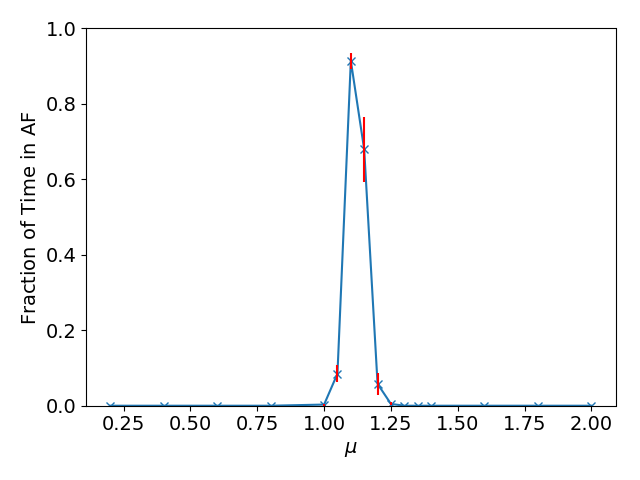
\includegraphics{risk_curve_3}
    \caption{The risk curve for the generalised model. Above $\mu \approx 1.25$, there is no fibrillation because the network is so well-connected that re-entry circuits are `shorted out'. Below $\mu \approx 1.00$ there is no fibrillation because there is no propagation at all; the signal dies out a short distance from the sinoatrial node. Note that each point represents the mean fraction of time in fibrillation for 1000 networks. Error bars are calculated using the $3 \times$ the standard error of the mean of the fractional time spent in AF, otherwise they would not be visible.}
    \label{fig:ourriskcurve}
\end{mdframed} \end{figure}

\clearpage

\subsection{Conduction Anisotropy}

The conduction velocity along fibres should be greater than the conduction velocity perpendicular to the fibres. In order to test this, an isotropic (or `null') model was created. The procedure to do this was as follows:
\begin{enumerate}
    \item Create an empty region containing no cells, of the same size as the region containing the original (`anisotropic') model.
    \item For every voxel in the original map that contains a cell, add a cell to this new model. This ensures that the null model has the same shape as the original.
    \item Add connections between these cells as a function of distance between them using Eq.~\eqref{eq:pconn}.
\end{enumerate}
This is enough to create a model that lacks the overall anisotropy of the sheep heart model, but otherwise looks very similar. We would expect the way the signal propagates through this model to be qualitatively different to the way it propagates through the real model. The result of running the model and measuring the time at which each cell is first activated is shown in Fig.~\ref{fig:activationtimes}. We see that we get the qualitative difference we expect.
Note that Fig.~\ref{fig:activationtimes} is derived from only a single network of the 1,000.

\begin{figure}[h] \begin{mdframed}
    \centering
    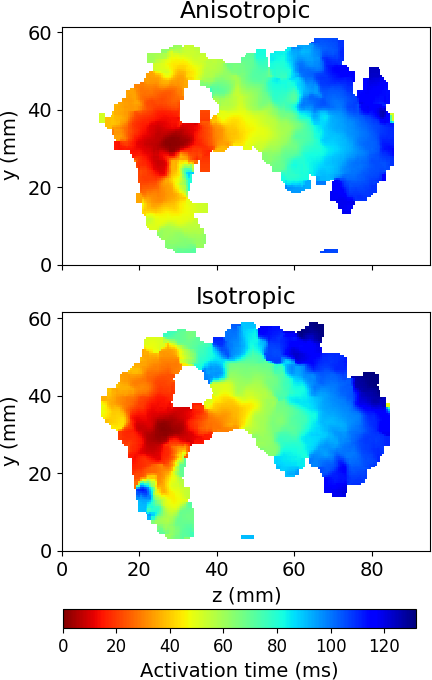
\includegraphics{activation_times_smooth}
    \caption{Time at which each cell in the model is first activated. This is a view of a quasi-two-dimensional slice through the heart. It can be seen that the activation patterns are qualitatively different, differing most noticeably in when the signal reaches the left atrium. We also see that the anisotropic model is much smoother, with fewer patches that are activated much later than their neighbours than in the isotropic case. The slight differences in shape of the two atria are caused by artefacts of the way the visualisation is generated and are not biologically relevant.}
    \label{fig:activationtimes}
\end{mdframed} \end{figure}

\clearpage

\subsection{Re-entry Circuit Distribution}

Our algorithm to find re-entry circuits in the original CMP model (see Fig.~\ref{fig:reentryalgo}) was used to find re-entry circuits in the sheep heart model. We designed this algorithm to work on a general network, so adapting it to this more complex substrate was a straightforward task. The spatial distribution of re-entry circuits in our model is shown in Fig.~\ref{fig:af_heatmap}.

It can be seen that the re-entry circuits mostly cluster around the sleeves of the pulmonary veins, with some re-entrant activity on the left atrial appendage and posterior left atrium; this is consistent with clinical observations~\cite{ehrlich2003cellular}. With increased fibrosis (corresponding to lower $\mu$) the area at risk of re-entrant activity increases, and correspondingly the risk of AF increases. This could explain why ablation strategies are less effective in persistent atrial fibrillation; if increased fibrosis results in more persistent fibrillation, and also increases the number of risk areas, the chance of destroying all re-entry circuits with an ablation becomes less favourable.

Most importantly, this highlights areas that have been implicated in drivers of AF by clinical studies, suggesting that regions of AF are in part caused by the fibre orientation in the atrium.

\begin{figure} \begin{mdframed}
    \begin{subfigure}[b]{0.92\textwidth}
        \centering
        \includegraphics[width=\textwidth]{{af_heatmap_mu=1.15_redo}.png}
        \caption{$\mu=1.15$}
    \end{subfigure}

    \begin{subfigure}[b]{0.92\textwidth}
        \centering
        \includegraphics[width=\textwidth]{{af_heatmap_mu=1.1_redo}.png}
        \caption{$\mu=1.1$}
    \end{subfigure}
    \caption{The probability of re-entry circuits over the surface of the atrium. Anything with a risk under 25\% is shown in grey for contrast. There is an increased risk of re-entry circuits on the sleeves of the pulmonary veins, especially the right superior pulmonary vein (RSPV on diagram), the left atrial appendage (LAA) and the posterior left atrium (PLA). It can be seen that as $\mu$ decreases, the risk regions increase in size and number, spreading to the right atrial appendage (RAA) and across the surface.}
    \label{fig:af_heatmap}
\end{mdframed} \end{figure}

\clearpage

\subsection{Harmonic Centrality}

The circuit finding algorithm was computationally intensive so a proxy was sought. The process applied here was almost identical to the process described in Sec.~\ref{sec:centrality}; re-entry circuits form in the same way as before so we would expect harmonic centrality to predict them effectively. When calculating $H_i$ we neglected summation terms where $d_{ij}$ was larger than 20. The calculated centrality was compared with the distribution of re-entry circuits. The results are shown in Fig.~\ref{fig:newcentrality}.

Centrality is a poor predictor of re-entrant activity in this model, which means that we have failed to find a computationally inexpensive proxy for re-entry. This may be because re-entry circuits in this model are much more complicated so they do not involve stretches of isolated fibre as they did in the CMP model. Additionally, large-scale heterogeneity makes the approximation used when calculating $H_i$ less valid than it was for the CMP model.

\begin{figure}[h] \begin{mdframed}
    \centering
    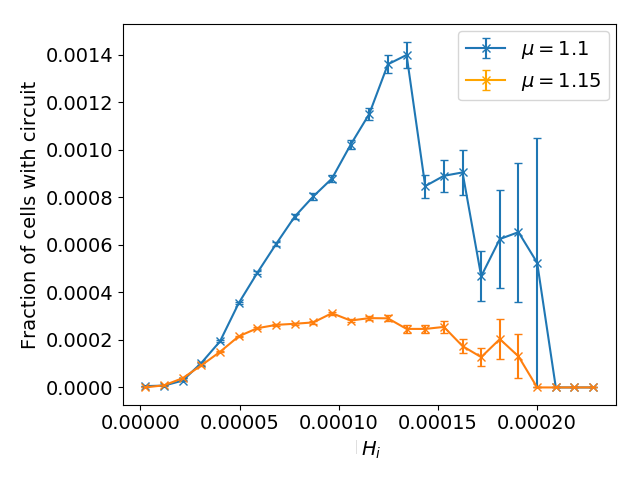
\includegraphics{circuits_vs_centrality_3}
    \caption{$H_i$ plotted against the probability of a circuit. It can be seen that harmonic centrality is no longer a useful predictor of re-entrant activity. Though the data is binomial (as each cell either has a circuit or not), there are many points in each bin so a Gaussian approximation was used to calculate the standard error of the mean for the error bars.}
    \label{fig:newcentrality}
\end{mdframed} \end{figure}

\clearpage


\section{Implementation}

As before, the model was written in C++ and Python using the Python/C API for the high-performance of C++ and the flexibility and libraries of Python. 

We were able to make use of Imperial's high performance computing cluster, allowing us to simulate 1000 networks per value of $\mu$. In order to achieve compatibility with Imperial's high performance computing facilities, much of the C++ had to be rewritten to an older standard. However, to simply run the model for a single heart, consumer hardware was more than sufficient.

We implemented from scratch every algorithm listed in this section, as well as the model itself. This required 6304 lines of code in total, with 3851 being C++ code required to run the simulation and another 2425 lines of Python code for data analysis or visualisation. We used no external libraries other than the standard Python libraries, Matplotlib, and NumPy.

We used several techniques to improve performance, besides improvements to the algorithmic complexity already mentioned. We duplicated many of the improvements discussed for the CMP model (Sec.~\ref{sec:cmpimpl}), such as profiling, and applying the cell update algorithm to only excited cells and their neighbours. 
% The model was implemented as a set of node objects which stored their state information and kept pointers to their neighbours, which meant that propagating signals through the model was much faster than implementations using other common ways to store networks.

\section{Key Points from Chapter \thechapter}

\begin{itemize}
    \item We have developed a procedure to turn a vector field representing the fibre orientation in a sheep atrium into a network model of the heart, where cells are not tied to a lattice. This procedure is computationally intensive but reduces density bias more than any other procedure we devised.
    \item We have a control parameter $\mu$ which is analogous to fibrosis in the real heart, and analogous to the control parameter $\nu$ from the CMP model. We find that the risk of atrial fibrillation varies in the expected way when we vary $\mu$, providing a necessary verification of the model's correctness.
    \item Our isotropic and anisotropic conduction models show qualitatively different behaviour, as expected and as shown in other models~\cite{zhao}.
    \item Harmonic centrality fails to predict re-entry on this generalised model.
    \item We find that the distribution of re-entry circuits in our model has good agreement with the clinically measured distribution, and that decreasing $\mu$ results in a larger risk area.
\end{itemize}
